% \documentclass[lineno,twocolumn,endfloat,biblatex]{biophys-new}
\documentclass{biophys-new}
\usepackage[utf8]{inputenc}
\usepackage{graphicx}
\usepackage[colorlinks,allcolors=cyan!70!black]{hyperref}
\usepackage{glossaries}
\usepackage{textcomp}
\usepackage{subcaption}
\usepackage{comment}
\usepackage{tabularx}
\usepackage{subcaption}
\usepackage{datatool}
\usepackage{booktabs}
\usepackage{etoolbox}
\newcommand{\rev}[1]{{\color{blue} #1}}
% Uncomment if using biblatex
% \addbibresource{sample.bib}
\newacronym{nka}{NKA}{sodium-potassium ATPase pump}
\title{Model comparison and system analysis of Na+/K+-ATPase using bond graph}
\runningtitle{Biophysical Journal Template} %% For page header

\author[1,*]{First author}
\author[2]{Second author}
\runningauthor{Author1 and Author2} %% For page header

\affil[1]{Institution A, Address A}
\affil[2]{Institution B, Address B}

\corrauthor[*]{abx@xyz.edu}

% \papertype{Letters}
\papertype{Article}
% \papertype{Computational Tools}

% Define a custom command to generate tables from CSVs
% #1 = CSV filename, #2 = Caption, #3 = Label (also used as unique DB name)
\newcommand{\makeparametertable}[3]{%
    % 1. Load data into a unique database named after the label (#3)
    \DTLloadrawdb[
      keys={u_0_Vm,c_Nai,c_Nao,c_Ki,c_Ko,c_Pi,c_ATP,c_ADP,T,pH,v_ss}
    ]{#3}{#1}
    
    % 2. Clear and build the macro for the table body
    \def\mytablebody{}
    \DTLforeach*{#3}{%
      \cola=u_0_Vm,\colb=c_Nai,\colc=c_Nao,\cold=c_Ki,\cole=c_Ko,\colf=c_Pi,\colg=c_ATP,\colh=c_ADP,\coli=T,\colj=pH,\colk=v_ss%
    }{%
      \eappto\mytablebody{\cola & \colb & \colc & \cold & \cole & \colf & \colg & \colh & \coli & \colj & \colk \noexpand\\}%
    }
    
    % 3. Print the table
    \begin{table}[htbp]
    \centering
    \begin{tabularx}{\textwidth}{ 
      >{\raggedright\arraybackslash}X 
      >{\centering\arraybackslash}X 
      >{\centering\arraybackslash}X 
      >{\centering\arraybackslash}X 
      >{\centering\arraybackslash}X 
      >{\centering\arraybackslash}X 
      >{\centering\arraybackslash}X 
      >{\centering\arraybackslash}X 
      >{\centering\arraybackslash}X 
      >{\centering\arraybackslash}X 
      >{\centering\arraybackslash}X 
    }
    \toprule
    $V_m$(V) & $c_{Nai}$ (mM) & $c_{Nao}$ (mM) & $c_{Ki}$ (mM) & $c_{Ko}$ (mM) & $c_{Pi}$ (mM)& $c_{ATP}$ (mM)& $c_{ADP}$ (mM) & T (K) & pH & $v$ (fmol/s) \\
    \midrule
    \mytablebody
    \bottomrule
    \end{tabularx}
    \caption{#2}
    \label{#3}
    \end{table}
}

\begin{document}


\section*{Introduction}

This document includes the detailed model description of the \Gls{nka} used in the main paper. 


\section*{Methods}

\subsection*{Bond graph model of \Gls{nka} with 15 states}

The reaction scheme can be found in the paper \cite{pan_cardiac_2020}, while we redraw the bond graph in Figure \ref{fig:15state} using the new notation.
\begin{figure}
\centering
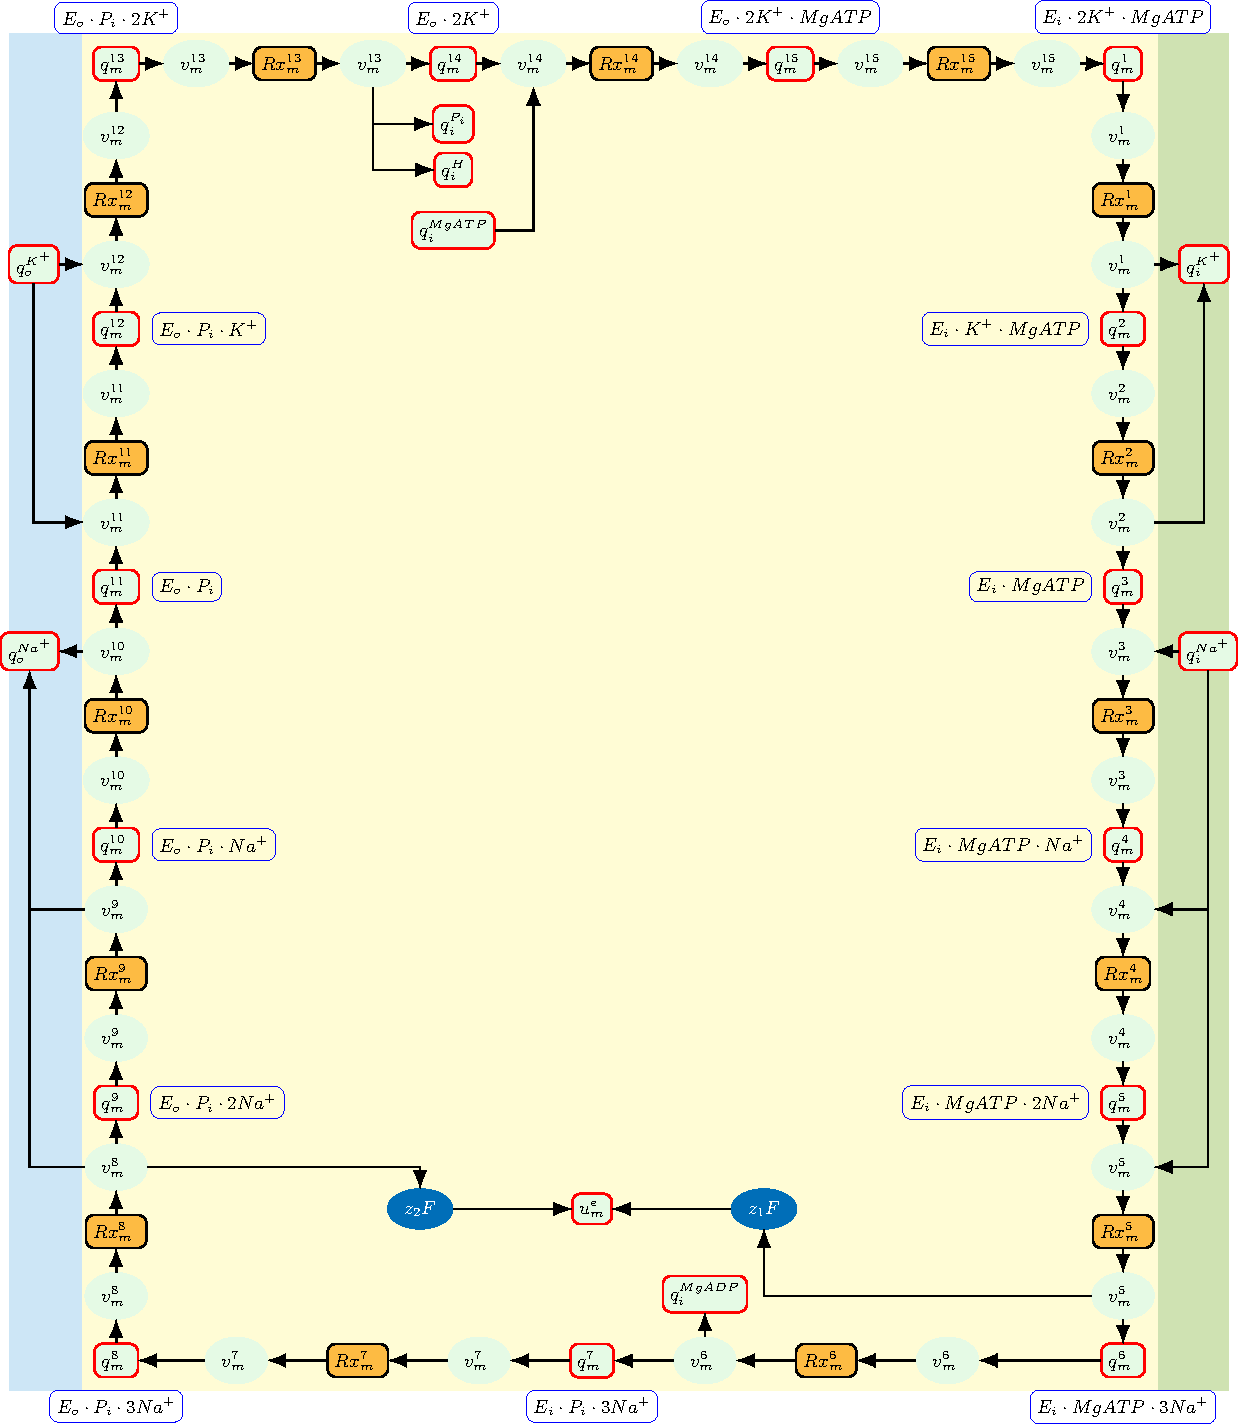
\includegraphics[width=0.9\linewidth]{15state.pdf}
\caption{Bond graph of the 15-state model, adapted from \cite{pan_cardiac_2020}.}
\label{fig:15state}
\end{figure}

\input{15state_eqs.tex}

The CellML code of the model is \textit{NKE\_BG\_15\_state.cellml} and the parameters are in \textit{NKE\_BG\_params.cellml},
while the file \textit{NKE\_BG\_Env.cellml} contains the environmental variables and the membrane potentials used in the simulation.
The simulation conditions are in the sedml files listed in \textit{NKE\_BG\_15\_state\_sedmls.json},
while the python scripts to edit and run the sedml files are: \textit{edit\_sedmls\_NKE\_BG\_15\_state.py} and \textit{run\_sedmls\_NKE\_BG\_15\_state.py}.

The steady state flux of the 15-state model is given in the CellML code \textit{Terkildsen\_NaK\_kinetic\_modular.cellml} associated with the paper \cite{pan_cardiac_2020}.
We modified the code to allow the model access to the environmental variables in \textit{NKE\_BG\_Env.cellml} and renamed it as \textit{Terkildsen\_NaK\_kinetic\_modular\_V.cellml}.
The simulation conditions are in the sedml files listed in \textit{Terkildsen\_NaK\_kinetic\_modular\_V\_sedmls.json},
while the python scripts to edit and run the sedml files are: \textit{edit\_sedmls\_Terkildsen\_NaK\_kinetic.py} and \textit{run\_sedmls\_Terkildsen\_NaK\_kinetic\_modular\_V.py}.

\subsection*{Bond graph modes of \Gls{nka} with 6 states}

The bond graph of the 6-state model is shown in Figure \ref{fig:6state_v1}.
\begin{figure}
\caption{Bond graph mode of \Gls{nka} with 6 states.}
      \label{fig:6state_v1}
\centering
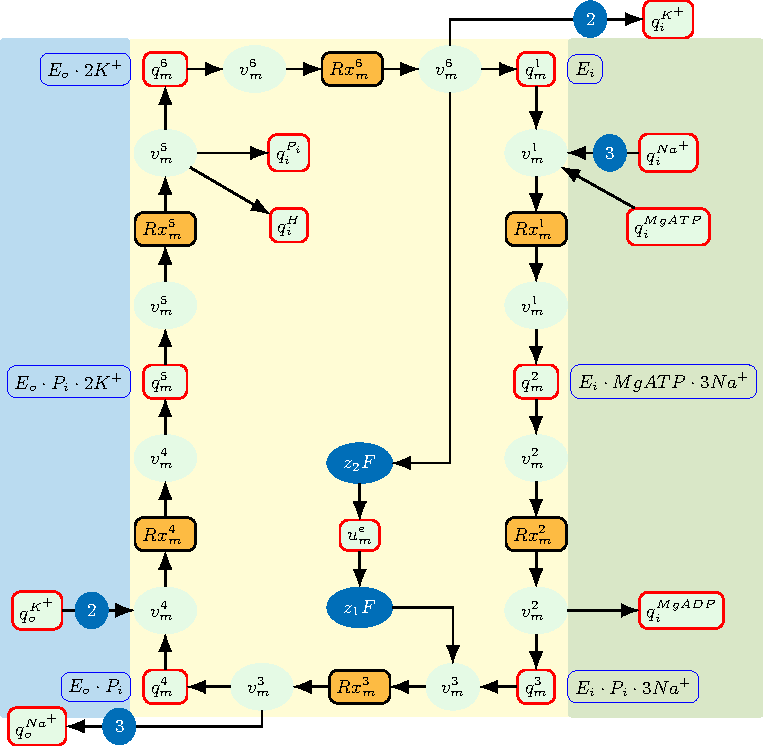
\includegraphics[width=0.7\linewidth]{6state_1.pdf}
\end{figure}

\input{6state_eqs.tex}

\rev{ The experimental conditions and corresponding data used for the parameter fitting process are listed from Table \ref{tab:volt_cond} to Table \ref{tab:ATP_cond}.}
% Generate the first table
\makeparametertable{Terkildsen_NaK_kinetic_volt_cond.csv}% File
                   {The boundary conditions for Fig 2b in \cite{pan_cardiac_2020}.}% Caption
                   {tab:volt_cond}% Label

\makeparametertable{Terkildsen_NaK_kinetic_Nai_cond.csv}% File
                   {The boundary conditions for Fig 3a in \cite{pan_cardiac_2020}.}% Caption
                   {tab:Nai_cond}% Label
\makeparametertable{Terkildsen_NaK_kinetic_Ke_cond.csv}% File
                   {The boundary conditions for Fig 3b in \cite{pan_cardiac_2020}.}% Caption
                   {tab:Ke_cond}% Label
\makeparametertable{Terkildsen_NaK_kinetic_ATP_cond.csv}% File
                   {The boundary conditions for Fig 3c in \cite{pan_cardiac_2020}.}% Caption
                   {tab:ATP_cond}% Label

Table \ref{tab:6state-params} lists the parameters used in the 6-state model.
\begin{table}[h]
\centering
\caption{Parameters used in the 6-state model.}
\label{tab:6state-params}
\begin{tabular}{l l l}
\hline
Parameter & Value & Unit \\
\hline
\hline
$\kappa_1$ & 62051.4 & $fmol \cdot s^{-1}$ \\
$\kappa_2$ & 0.549906 & $fmol \cdot s^{-1}$\\
$\kappa_3$ & 474.926& $fmol \cdot s^{-1}$ \\
$\kappa_4$ & 910019 & $fmol \cdot s^{-1}$ \\
$\kappa_5$ & 384.851& $fmol \cdot s^{-1}$ \\
$\kappa_6$ & 3412.49 & $fmol \cdot s^{-1}$ \\
$K_1$ & 3.64797 & $fmol^{-1}$ \\
$K_2$ & 80.1178  & $fmol^{-1}$ \\
$K_3$ & 99322.9 & $fmol^{-1}$ \\
$K_4$ & 49.0681  & $fmol^{-1}$ \\
$K_5$ & 84.2138 & $fmol^{-1}$ \\
$K_6$ & 727440 & $fmol^{-1}$ \\
$z_1$ & 0.945049 & dimensionless \\
$z_2$ & -0.054951 & dimensionless \\
\hline
\end{tabular}
\end{table}

% Table file name, description of the file
Table \ref{tab:6state-files} lists and describes the files related to the 6-state model.
\begin{table}
\centering
\caption{Description of the files related to the 6-state model.}
\label{tab:6state-files}
\begin{tabularx}{\linewidth}{p{8cm} X }
\hline
File name & Description \\
\hline
\hline
\textit{NKE\_BG\_6\_state\_ATPNaZKV2.cellml} & CellML code of the 6-state model \\
\textit{NKE\_BG\_6\_state\_ATPNaZKV2\_SS.cellml} & CellML code of the steady state flux of the 6-state model \\
\textit{NKE\_BG\_6\_state\_ATPNaZKV2\_fixedV.cellml} & CellML code of the 6-state model with fixed membrane potential \\
\textit{NKE\_BG\_6\_state\_ATPNaZKV2\_SS\_fixedV.cellml} & CellML code of the steady state flux of the 6-state model with fixed membrane potential \\
\textit{NKE\_BG\_6\_state\_ATPNaZKV2\_param.cellml} & Parameters for the 6-state model \\
\textit{NKE\_BG\_6\_state\_ATPNaZKV2\_sedmls.json} & The list of sedml files for the 6-state model \\
\textit{NKE\_BG\_6\_state\_ATPNaZKV2\_fixedV\_sedmls.json} & The list of sedml files for the 6-state model with fixed membrane potential \\
\textit{NKE\_BG\_6\_state\_ATPNaZKV2\_SS\_sedmls.json} & The list of sedml files for the steady state flux of the 6-state model \\
\textit{NKE\_BG\_6\_state\_ATPNaZKV2\_SS\_fixedV\_sedmls.json} & The list of sedml files for the steady state flux of the 6-state model with fixed membrane potential \\
\textit{edit\_sedmls\_NKE\_BG\_6\_state\_ATPNaZKV2.py} & Python script to edit the sedml files for the 6-state model \\
\textit{run\_sedmls\_NKE\_BG\_6\_state\_ATPNaZKV2.py} & Python script to run the sedml files for the 6-state model \\
\hline
\end{tabularx}     
\end{table}

\subsection*{Instructions to run the simulations and reproduce the figures}

The CellML and sedml files are in workspace \url{https://models.physiomeproject.org/workspace/cad}, while the python scripts are in Github repository \url{https://github.com/WeiweiAi/EA_NKE}.
Since the Github repository includes sumbodules, please clone the repository using the command:
\begin{verbatim}
git clone https://github.com/WeiweiAi/EA_NKE.git --recurse-submodules
\end{verbatim}
It is recommended to use Python version 3.11. Please create a virtual environment and install the required packages using the command:
\begin{verbatim}
pip install -r requirements.txt
\end{verbatim}
Please move to the scripts directory: \textit{cd scripts} and the procedures to run the simulations and reproduce the figures are described below:
\begin{enumerate}
    \item \textit{python run\_sedmls\_Terkildsen\_kinetic.py} to get the data of the steady state flux of the 15-state model under varying conditions.
    \item \textit{python run\_sedmls\_NKE\_BG\_15\_state.py} to get the data of the full bond graph of the 15-state model under varying conditions.
    \item \textit{python run\_sedmls\_NKE\_BG\_6\_state\_ATPNaZKV2.py} to run the simulations of the 6-state models under varying conditions.
    \item \textit{python EA\_calc\_6stateV2.py} to calculate the energetic quantities of the 6-state model under varying conditions.
    \item \textit{python EA\_calc\_15state.py} to calculate the energetic quantities of the 15-state model under varying conditions.
    \item \textit{python plot\_original\_ssV2.py} to reproduce Figure 4 in the main paper.
    \item \textit{python plot\_EA\_flow\_6stateV2.py}, \textit{python plot\_EA\_flow\_15state.py} and \textit{python plot\_EA\_bar\_heatV2.py} to reproduce Figure 5 in the main paper.
    \item \textit{python plot\_EA\_2D\_combine15state\_2.py} and \textit{python plot\_EA\_2D\_combine6stateV2\_2.py} to reproduce Figure 6 in the main paper.
    \item \textit{python plot\_EA\_2D\_combine15state\_deltaATP\_2.py} and \textit{python plot\_EA\_2D\_combine6stateV2\_deltaATP\_2.py} to reproduce Figures 7,8 and 9 in the main paper.
    \item \textit{python plot\_EA\_2D\_combine15state\_flowRate\_2.py} and \textit{python plot\_EA\_2D\_combine6stateV2\_flowRate\_2.py} to reproduce Figure 10 in the main paper. 
    \item \textit{python plot\_EA\_2D\_combine15state\_NaK\_2.py} and \textit{python plot\_EA\_2D\_combine6stateV2\_NaK\_2.py} to reproduce Figure 11 in the main paper.  
\end{enumerate}  

\subsection*{Figures with more BCL options}
\rev{The extra figures with BCL = 600, 800, 1000, 1200 ms are shown below, and the scripts to plot the figures are:
\begin{enumerate}
 \item \textit{python plot\_EA\_2D\_combine15state.py} and \textit{python plot\_EA\_2D\_combine6stateV2.py} to reproduce Figure \ref{fig:thermodynamic_efficiency_AP}.
    \item \textit{python plot\_EA\_2D\_combine15state\_deltaATP.py} and \textit{python plot\_EA\_2D\_combine6stateV2\_deltaATP.py} to reproduce Figures \ref{fig:thermodynamic_efficiency_AP_deltaGATP},\ref{fig:electrical_efficiency_AP_deltaGATP} and \ref{fig:Mean_flow_rate_AP_deltaGATP}.
    \item \textit{python plot\_EA\_2D\_combine15state\_flowRate.py} and \textit{python plot\_EA\_2D\_combine6stateV2\_flowRate.py} to reproduce Figure \ref{fig:thermodynamic_efficiency_AP_flowRate}. 
    \item \textit{python plot\_EA\_2D\_combine15state\_NaK.py} and \textit{python plot\_EA\_2D\_combine6stateV2\_NaK.py} to reproduce Figure \ref{fig:thermodynamic_efficiency_AP_NaK}.
\end{enumerate}
}
\begin{figure}[htbp]
\centering
\begin{subfigure}{0.48\textwidth}
      \centering  
      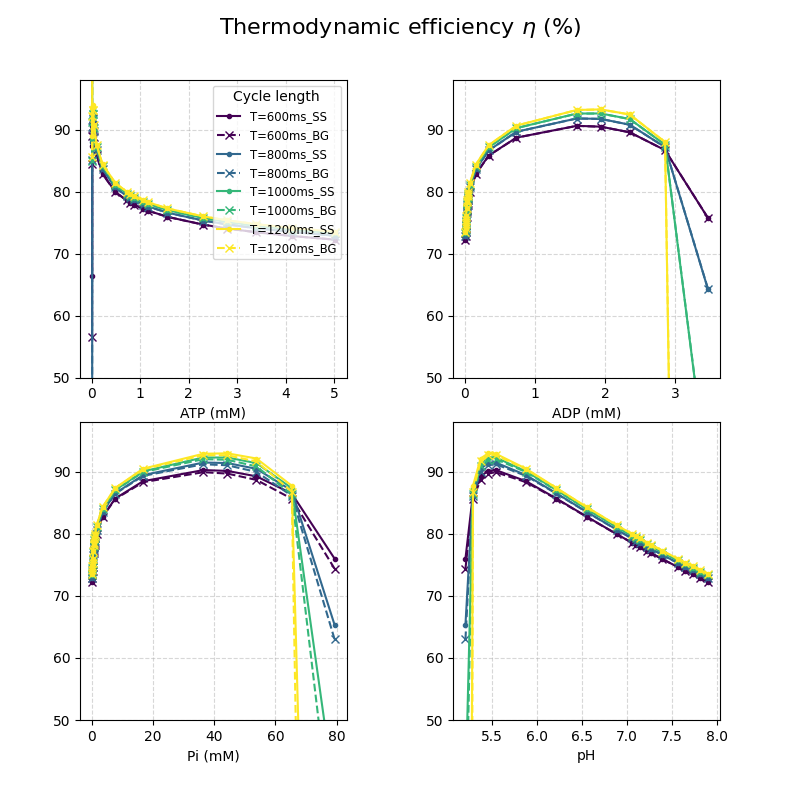
\includegraphics[width=\linewidth]{EA_2D_combine_6stateV2_Thermodynamic_efficiency.png}
      \caption{6-state model}    
\end{subfigure}
\begin{subfigure}{0.48\textwidth}
      \centering
      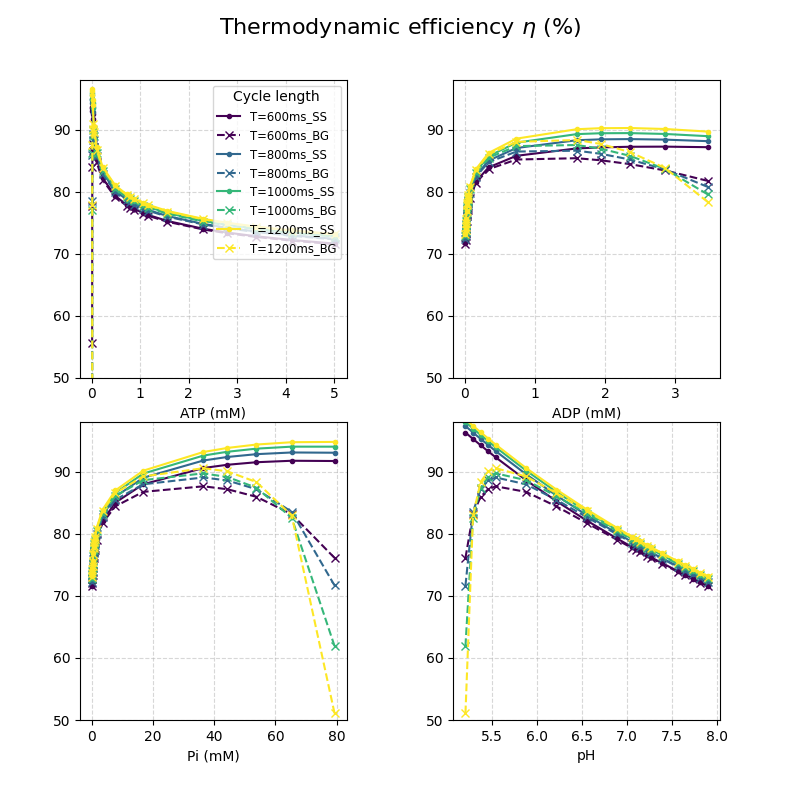
\includegraphics[width=\linewidth]{EA_2D_combine_15state_Thermodynamic_efficiency.png}  
      \caption{15-state model}    
\end{subfigure}
\caption{Thermodynamic efficiency of \gls{nka} (a) (6-state model) and (b) (15-state model).}
\label{fig:thermodynamic_efficiency_AP} 
\end{figure} 

\begin{figure}[htbp]
\centering
\begin{subfigure}{0.4\textwidth}
      \centering  
      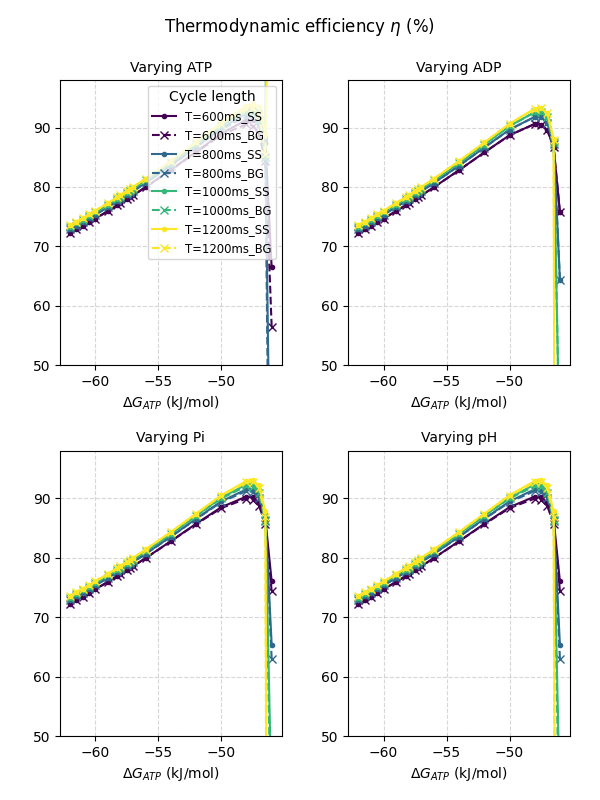
\includegraphics[width=\linewidth]{EA_2D_combine_6stateV2_Thermodynamic_efficiency_deltaATP.png}
      \caption{6-state model}    
\end{subfigure}
\begin{subfigure}{0.4\textwidth}
      \centering
      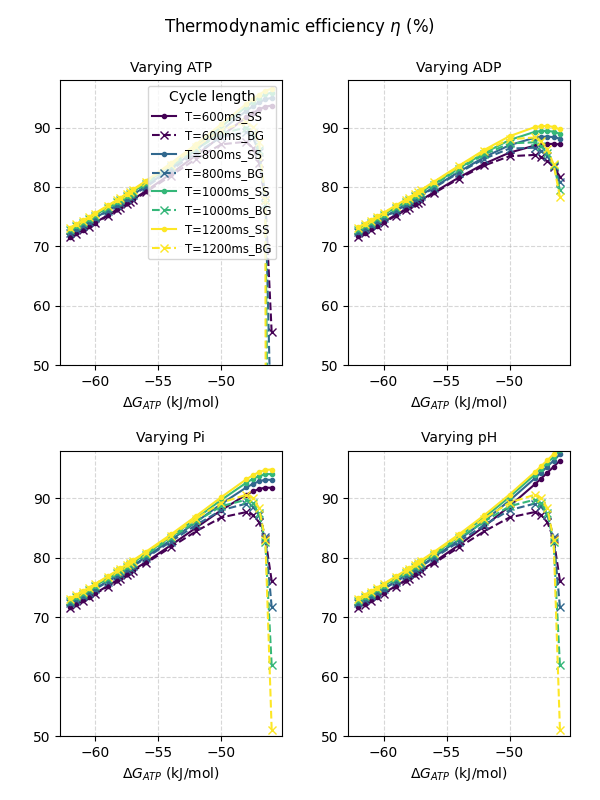
\includegraphics[width=\linewidth]{EA_2D_combine_15state_Thermodynamic_efficiency_deltaATP.png}  
      \caption{15-state model}    
\end{subfigure}
\caption{Thermodynamic efficiency of \gls{nka} (a) (6-state model) and (b) (15-state model) under different $\Delta G_{ATP}$ values.}
\label{fig:thermodynamic_efficiency_AP_deltaGATP} 
\end{figure}

\begin{figure}[htbp]
\centering
\begin{subfigure}{0.4\textwidth}
      \centering  
      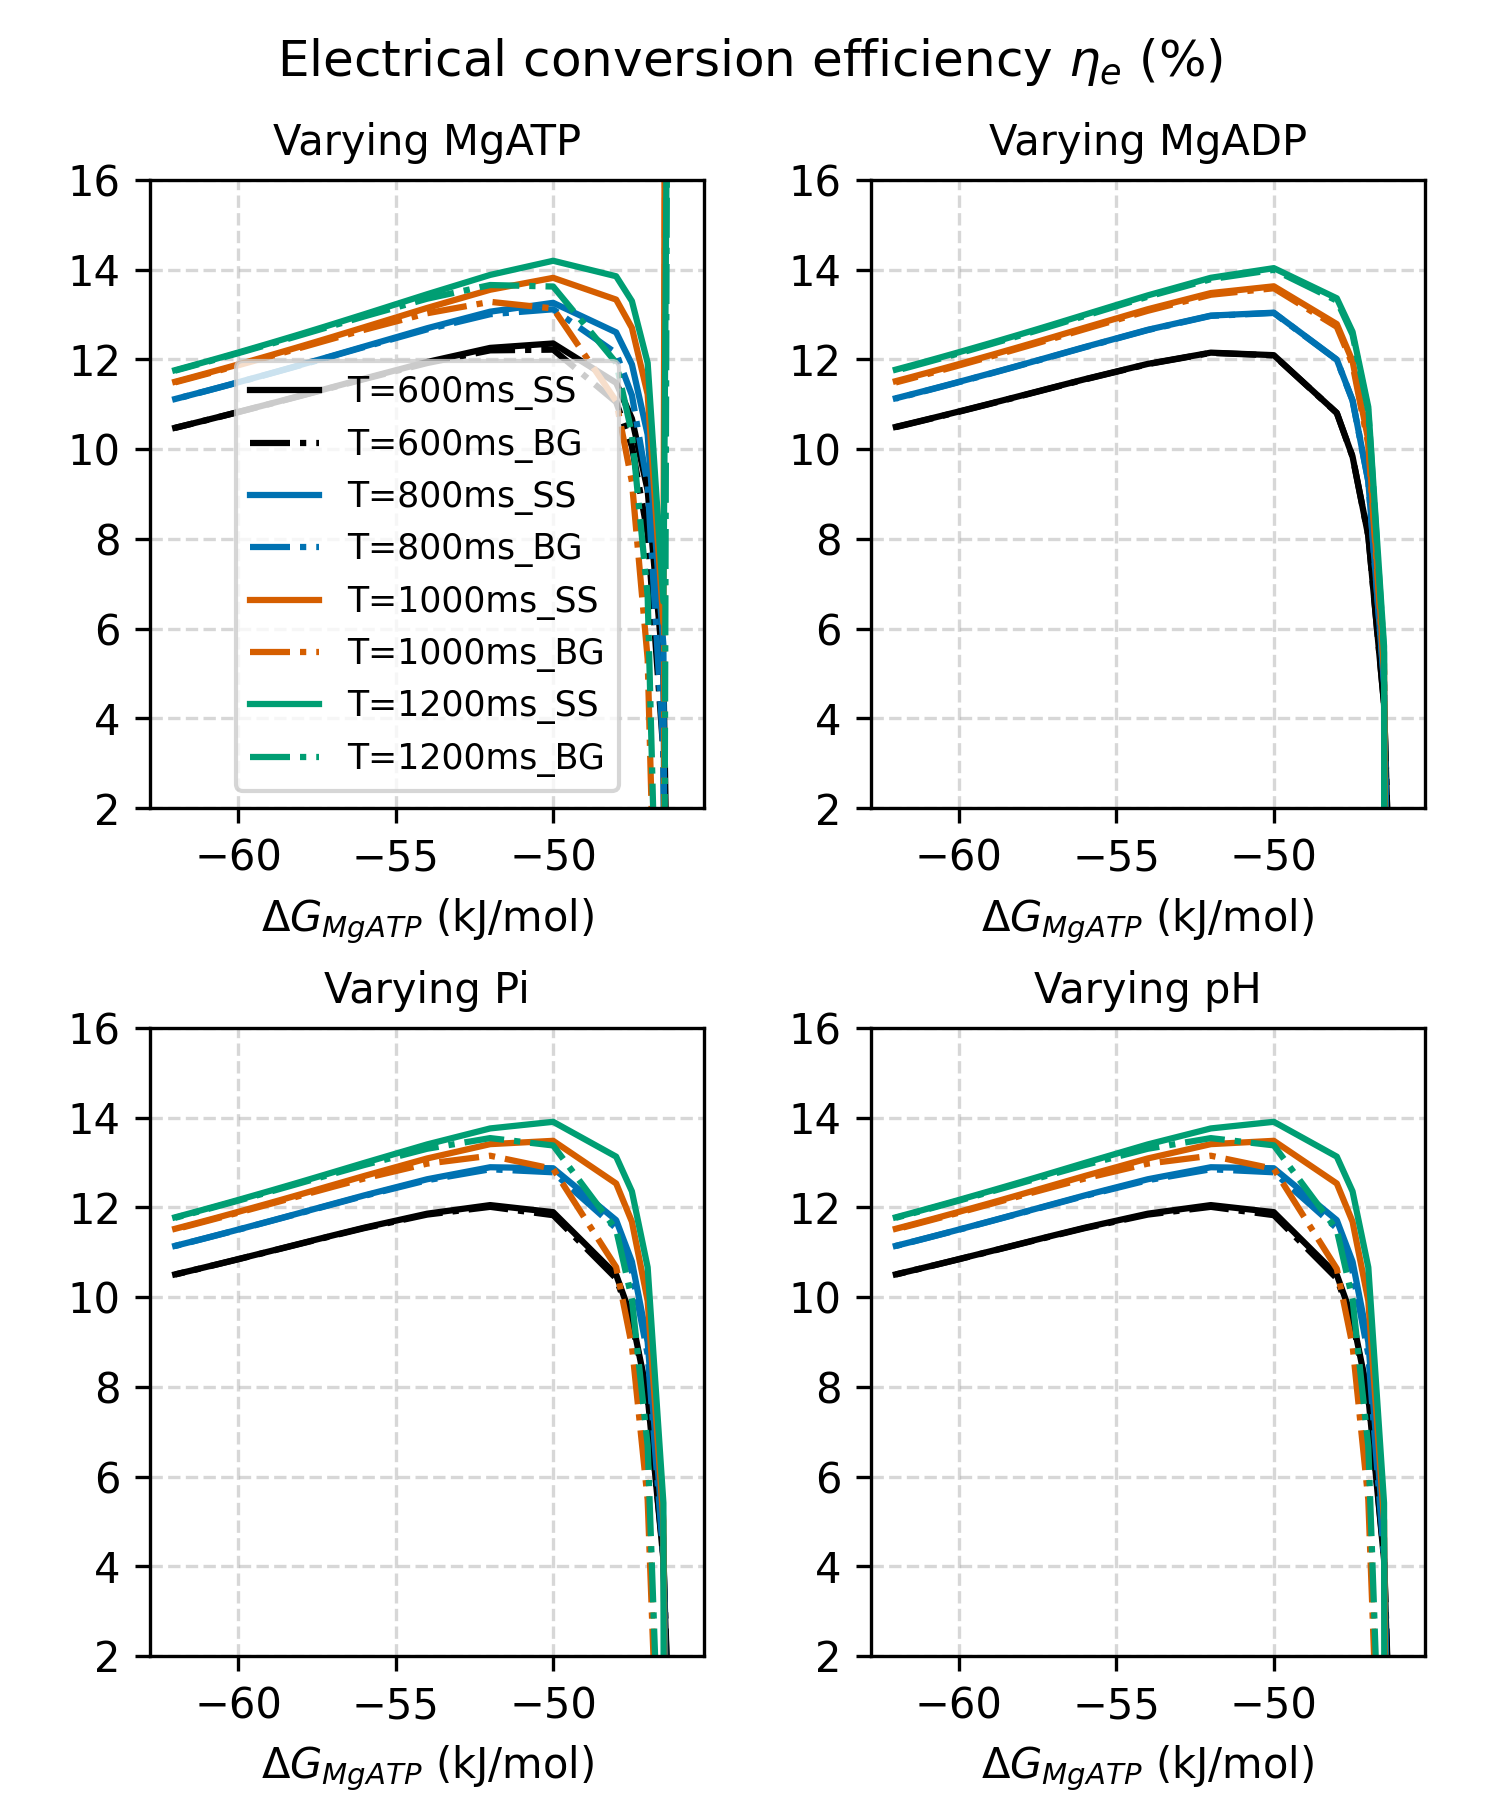
\includegraphics[width=\linewidth]{EA_2D_combine_6stateV2_Electrical_conversion_efficiency_deltaATP.png}
      \caption{6-state model}    
\end{subfigure}
\begin{subfigure}{0.4\textwidth}
      \centering
      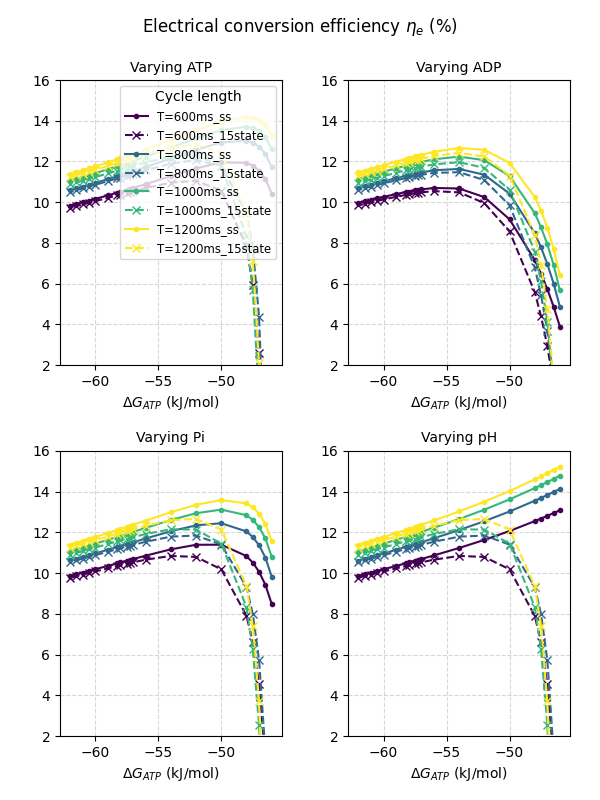
\includegraphics[width=\linewidth]{EA_2D_combine_15state_Electrical_conversion_efficiency_deltaATP.png}  
      \caption{15-state model}    
\end{subfigure}
\caption{Electrical conversion efficiency of \gls{nka} (a) (6-state model) and (b) (15-state model) under different $\Delta G_{ATP}$ values.}
\label{fig:electrical_efficiency_AP_deltaGATP} 
\end{figure}

\begin{figure}[htbp]
\centering
\begin{subfigure}{0.4\textwidth}
      \centering  
      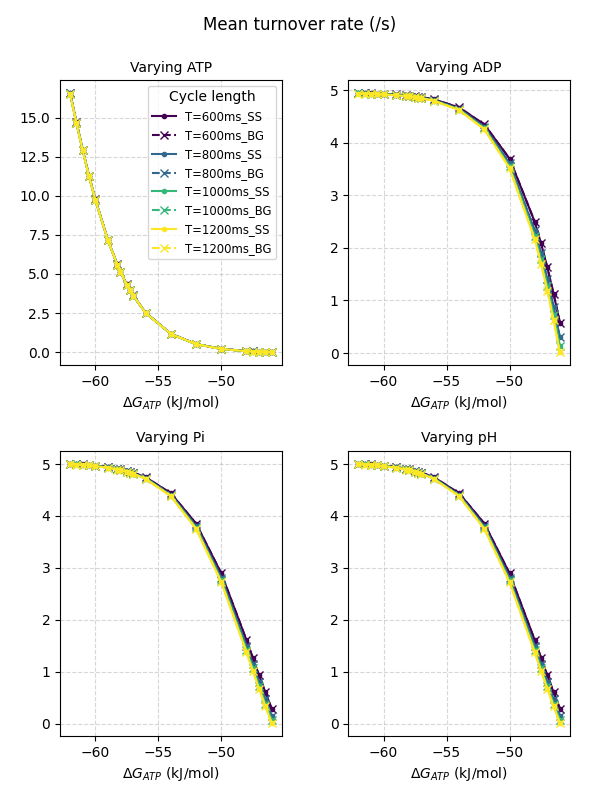
\includegraphics[width=\linewidth]{EA_2D_combine_6stateV2_Mean_flow_rate_deltaATP.png}
      \caption{6-state model}    
\end{subfigure}
\begin{subfigure}{0.4\textwidth}
      \centering
      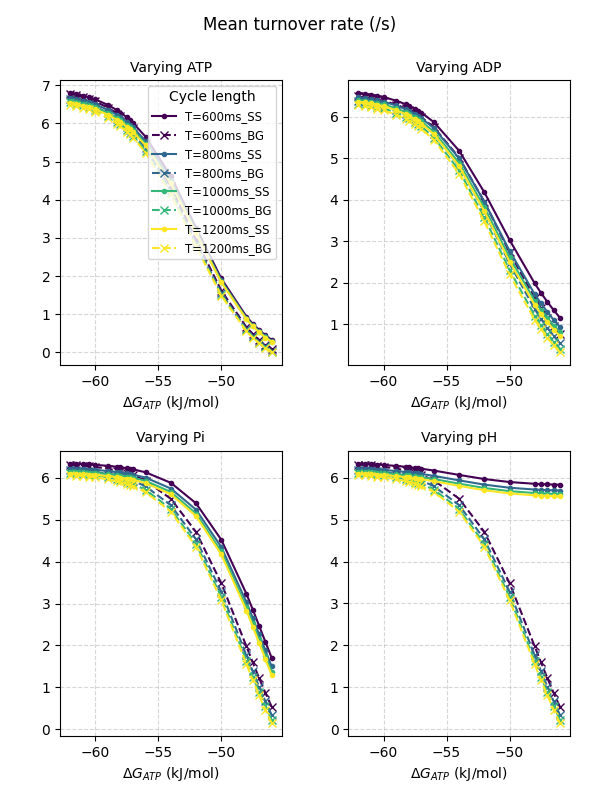
\includegraphics[width=\linewidth]{EA_2D_combine_15state_Mean_flow_rate_deltaATP.png}  
      \caption{15-state model}    
\end{subfigure}
\caption{Mean flow rate of \gls{nka} (a) (6-state model) and (b) (15-state model) under different $\Delta G_{ATP}$ values.}
\label{fig:Mean_flow_rate_AP_deltaGATP} 
\end{figure}

\begin{figure}[htbp]
\centering
\begin{subfigure}{0.4\textwidth}
      \centering  
      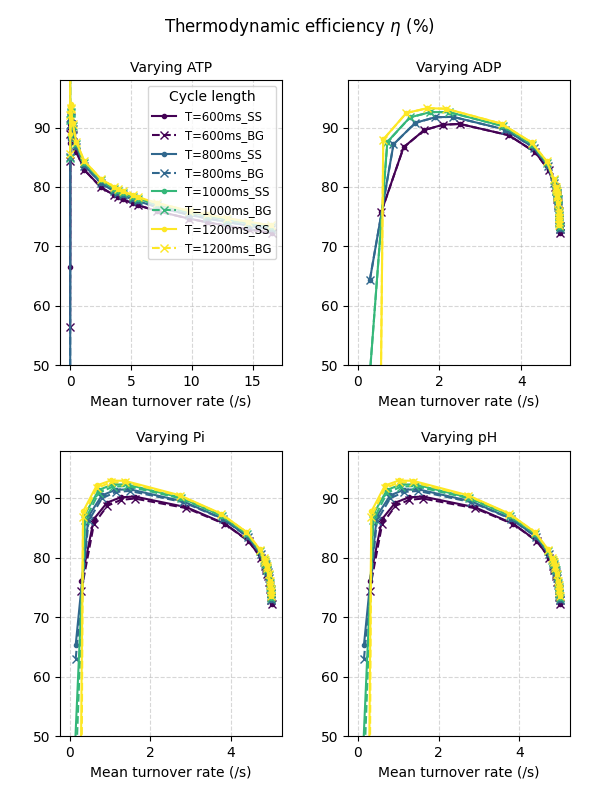
\includegraphics[width=\linewidth]{EA_2D_combine_6stateV2_Thermodynamic_efficiency_flowRate.png}
      \caption{6-state model}    
\end{subfigure}
\begin{subfigure}{0.4\textwidth}
      \centering
      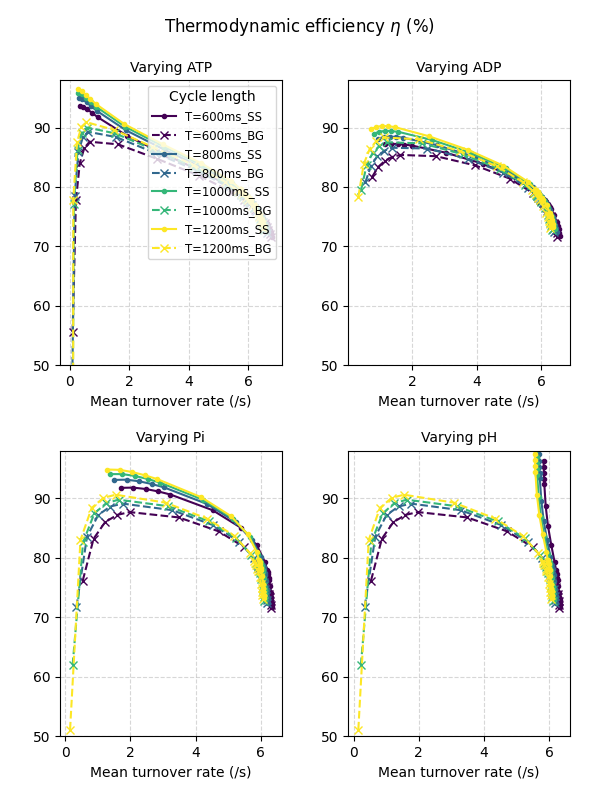
\includegraphics[width=\linewidth]{EA_2D_combine_15state_Thermodynamic_efficiency_flowRate.png}  
      \caption{15-state model}    
\end{subfigure}
\caption{Thermodynamic efficiency of \gls{nka} (a) (6-state model) and (b) (15-state model) under different mean turnover rates.}
\label{fig:thermodynamic_efficiency_AP_flowRate} 
\end{figure}

\begin{figure} [htbp]
\centering
\begin{subfigure}{0.4\textwidth}
      \centering  
      \includegraphics[width=\linewidth]{EA_2D_combine_6stateV2_Thermodynamic_efficiency_Nak.png}
      \caption{6-state model}    
\end{subfigure}
\begin{subfigure}{0.4\textwidth}
      \centering
      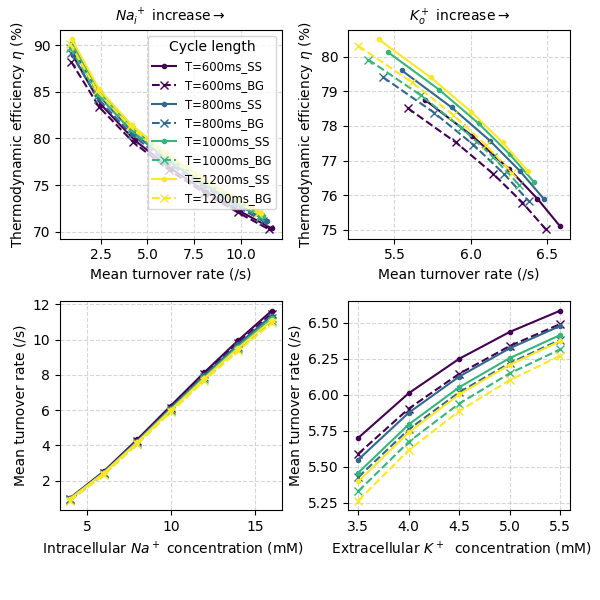
\includegraphics[width=\linewidth]{EA_2D_combine_15state_Thermodynamic_efficiency_NaK.png}  
      \caption{15-state model}    
\end{subfigure}
\caption{Thermodynamic efficiency and mean turnover rate of \gls{nka} (a) (6-state model) and (b) (15-state model) under different intracellular Na\textsuperscript{+} and extracellular K\textsuperscript{+} concentrations. The left panels of (a) and (b) show the thermodynamic efficiency of \gls{nka} with increased  mean turnover rate due to increased intracellular Na\textsuperscript{+} concentration, while the right panels of (a) and (b) show the thermodynamic efficiency of \gls{nka} with increased  mean turnover rate due to decreased extracellular K\textsuperscript{+} concentration.}
\label{fig:thermodynamic_efficiency_AP_NaK}
\end{figure}
\subsection*{Parameters used in the 6-state model for enterocyte simulation}

\begin{table}[h]
\centering
\caption{Parameters used in the 6-state model for enterocyte simulation.}
\label{tab:6state-paramsV3}
\begin{tabular}{l l l}
\hline
Parameter & Value & Unit \\
\hline
\hline
$\kappa_1$ & 2838.89 & $fmol \cdot s^{-1}$ \\
$\kappa_2$ & 51.10 & $fmol \cdot s^{-1}$\\
$\kappa_3$ & 469.35& $fmol \cdot s^{-1}$ \\
$\kappa_4$ & 619068.3 & $fmol \cdot s^{-1}$ \\
$\kappa_5$ & 35.87& $fmol \cdot s^{-1}$ \\
$\kappa_6$ & 868.36 & $fmol \cdot s^{-1}$ \\
$K_1$ & 0.01673 & $fmol^{-1}$ \\
$K_2$ & 4477.02  & $fmol^{-1}$ \\
$K_3$ & 46639.87 & $fmol^{-1}$ \\
$K_4$ & 720.58  & $fmol^{-1}$ \\
$K_5$ & 1.6069 & $fmol^{-1}$ \\
$K_6$ & 30254.3 & $fmol^{-1}$ \\
$z_1$ & 0.945049 & dimensionless \\
$z_2$ & -0.054951 & dimensionless \\
\hline
\end{tabular}
\end{table}
% Uncomment if using bibtex (default)
\bibliography{sample}

% Uncomment if using biblatex
% \printbibliography

\end{document}
